% Shared style for all Git & GitHub lectures (same look as the N-body course)
\documentclass[11pt,a4paper]{article}
\usepackage[margin=2.3cm]{geometry}
\usepackage[T1]{fontenc}
\usepackage{lmodern}
\usepackage{upquote}   % straight quotes in monospaced text, so commands can be copied
\usepackage{microtype}
% keep '--' as two real hyphens in monospace text (commands like --version)
\DisableLigatures[-,<,>]{family=tt*}
\usepackage{booktabs,enumitem,graphicx,xcolor}
\usepackage{array}
\usepackage{needspace}
\usepackage{longtable}
\usepackage{float}
\usepackage{tikz}
\usetikzlibrary{arrows.meta,calc,positioning,decorations.pathreplacing,shapes.geometric,fit,backgrounds}
\usepackage[most]{tcolorbox}
\usepackage{listings}
\usepackage{fancyhdr}
\usepackage[colorlinks=true,linkcolor=blue!50!black,urlcolor=blue!50!black,citecolor=blue!50!black]{hyperref}

\setlength{\parindent}{0pt}
\setlength{\parskip}{0.6em}
\setlength{\abovecaptionskip}{4pt}
\usepackage[font=small,labelfont=bf]{caption}
\setlist{itemsep=0.2em,topsep=0.3em}

% ---------- colours ----------
\definecolor{cbg}{HTML}{F6F8FA}
\definecolor{ckw}{HTML}{0B5CAD}
\definecolor{ccm}{HTML}{6A737D}
\definecolor{cst}{HTML}{B5451B}
\definecolor{cpart}{HTML}{1F6FB2}
\definecolor{cheavy}{HTML}{C0392B}
\definecolor{cgreen}{HTML}{2E8B57}

% ---------- terminal listings ----------
% In a terminal session, lines starting with "$" are what YOU type.
% Everything else is what Git prints back.
\lstdefinestyle{term}{
  basicstyle=\ttfamily\small, backgroundcolor=\color{cbg},
  frame=single, rulecolor=\color{black!15}, showstringspaces=false,
  breaklines=true, columns=fullflexible, keepspaces=true,
  aboveskip=0.6em, belowskip=0.6em, xleftmargin=4pt, xrightmargin=4pt,
  literate={\$\ }{{\textcolor{cgreen}{\$\ }}}2,
  upquote=true
}
\lstset{style=term}
\newcommand{\code}[1]{\texttt{\small #1}}

% ---------- boxes ----------
\newtcolorbox{history}{colback=yellow!8,colframe=orange!60!black,
  title={History},fonttitle=\bfseries\small,left=4pt,right=4pt,top=2pt,bottom=2pt}
\newtcolorbox{quickfact}{colback=purple!4,colframe=purple!55!black,
  title={Quick fact},fonttitle=\bfseries\small,left=4pt,right=4pt,top=2pt,bottom=2pt}
\newtcolorbox{keyidea}{colback=blue!4,colframe=blue!50!black,
  title={Key idea},fonttitle=\bfseries\small,left=4pt,right=4pt,top=2pt,bottom=2pt}
\newtcolorbox{pitfall}{colback=red!4,colframe=red!55!black,
  title={Pitfall},fonttitle=\bfseries\small,left=4pt,right=4pt,top=2pt,bottom=2pt}
\newtcolorbox{tryit}{colback=teal!5,colframe=teal!55!black,
  title={Try it},fonttitle=\bfseries\small,left=4pt,right=4pt,top=2pt,bottom=2pt,breakable}
\newtcolorbox{homework}[1]{colback=green!4,colframe=green!40!black,
  title={Homework #1},fonttitle=\bfseries\small,left=4pt,right=4pt,top=2pt,bottom=2pt,
  breakable}
\newtcolorbox{goals}{colback=gray!6,colframe=gray!60!black,
  title={Learning goals},fonttitle=\bfseries\small,left=4pt,right=4pt,top=2pt,bottom=2pt}

% Solutions always start on a fresh page, behind a clear warning.
\newcommand{\solutionspage}{%
  \clearpage
  \begin{tcolorbox}[colback=red!6,colframe=red!60!black,halign=center]
    {\Large\bfseries Solutions}\\[0.3em]
    {\small Stop here if you have not tried the homework yet.\\
    Attempt every task first, run the checker, and only then read on.}
  \end{tcolorbox}
}

% ---------- Git diagram styles (TikZ) ----------
\tikzset{
  commit/.style={circle,draw=black!70,fill=blue!10,minimum size=7mm,inner sep=0pt,font=\scriptsize\ttfamily},
  newcommit/.style={commit,fill=orange!25,dashed},
  tag/.style={draw,rounded corners=2pt,font=\scriptsize\ttfamily,inner sep=2pt},
  branchtag/.style={tag,fill=green!15,draw=green!40!black},
  headtag/.style={tag,fill=yellow!30,draw=orange!70!black},
  remotetag/.style={tag,fill=purple!10,draw=purple!60!black},
  area/.style={draw,rounded corners,minimum height=11mm,minimum width=33mm,align=center,font=\small},
  cmdarrow/.style={->,thick,>=Stealth},
  link/.style={->,thick,>=Stealth,black!70},
}

% ---------- header ----------
\pagestyle{fancy}
\fancyhf{}
\renewcommand{\headrulewidth}{0.3pt}
\fancyfoot[C]{\thepage}
\newcommand{\lecturetitle}[3]{%
  \fancyhead[L]{\small\textit{Git \& GitHub from Zero}}
  \fancyhead[R]{\small Lecture #1}
  \begin{center}
    {\Large\bfseries Lecture #1}\\[0.4em]
    {\LARGE\bfseries #2}\\[0.4em]
    {\small #3}
  \end{center}
  \vspace{0.5em}
}

\tikzset{
  cbx/.style={draw,rounded corners,fill=blue!6,minimum width=1.9cm,minimum height=8mm,align=center,font=\scriptsize\ttfamily,inner sep=2pt},
  oldc/.style={cbx,fill=black!8,draw=black!45,dashed,text=black!55},
  goodc/.style={cbx,fill=green!18,minimum width=1.55cm},
  badc/.style={cbx,fill=red!15,minimum width=1.55cm},
  unkc/.style={cbx,fill=yellow!20,minimum width=1.55cm},
  obj/.style={draw,rounded corners,align=center,font=\scriptsize\ttfamily,inner sep=3pt,minimum height=7mm}}
\begin{document}
\lecturetitle{10}{Recovery and Under the Hood}{The reflog, \texttt{reset}, \texttt{stash}, \texttt{bisect}, the \texttt{.git} folder, and where to go next}

\begin{goals}
\begin{itemize}
  \item Recover ``lost'' commits with the reflog, and undo a bad reset, merge or rebase.
  \item Explain the three modes of \code{git reset} and use each safely.
  \item Park unfinished work with \code{git stash}.
  \item Find the commit that introduced a bug with \code{git bisect}.
  \item Describe what is inside \code{.git}: blobs, trees, commits, refs, and why IDs behave as they do.
  \item Choose the right command for a situation, and know where to learn more.
\end{itemize}
\end{goals}

\section{Git rarely loses what you committed}

By now you have used several commands that sound dangerous: \code{amend}, \code{rebase}, \code{force-with-lease}, \code{reset}. The good news of this last lecture is that, once something is \emph{committed}, Git almost never really loses it. Commits that no branch points to any more stay in the repository for weeks. The skill is knowing how to find them. (Work that was \emph{never} committed is different: \code{git restore} and \code{reset --hard} destroy it for good, as you learned in Lecture 3.)

We use a practice repository again, with no server this time. From the course folder:

\begin{lstlisting}
$ bash codeHints/L10/setup_demo10.sh
$ cd practice/demo10
$ git log --oneline
6529ff1 Add waffle recipe
9d18d71 Add crepe recipe
28a460c Add pancake recipe
143b77c Add README
\end{lstlisting}

(It also contains the branches \code{side} and \code{chain}, used later. To rebuild it: \code{cd ../..} and run the script with \code{--reset}.)

\section{The reflog: Git's flight recorder}

Imagine you want to undo your last two commits and type a command too eagerly (\code{git reset} is explained properly in the next section; for now: ``move \code{main} back two commits and make my files match''):

\begin{lstlisting}
$ git reset --hard HEAD~2
HEAD is now at 28a460c Add pancake recipe
$ git log --oneline
28a460c Add pancake recipe
143b77c Add README
\end{lstlisting}

The crepe and waffle commits have vanished from the log. Are they gone? No. \code{main} just points to an older commit; the two commits are still stored, only nothing leads to them:

\begin{figure}[H]
\centering
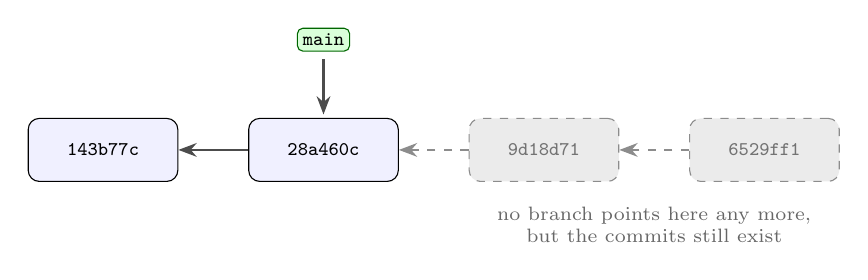
\begin{tikzpicture}
  \node[cbx] (a) at (0,0) {143b77c}; \node[cbx] (b) at (2.8,0) {28a460c};
  \node[oldc] (c) at (5.6,0) {9d18d71}; \node[oldc] (d) at (8.4,0) {6529ff1};
  \draw[link] (b)--(a); \draw[link,black!45,dashed] (c)--(b); \draw[link,black!45,dashed] (d)--(c);
  \node[branchtag] at (2.8,1.4) {main}; \draw[link] (2.8,1.15)--(2.8,0.45);
  \node[font=\scriptsize,anchor=north,text=black!60,align=center] at (7.0,-0.6) {no branch points here any more,\\but the commits still exist};
\end{tikzpicture}
\caption{After \code{reset --hard HEAD\textasciitilde{}2}. The branch label moved back; the two newer commits (dashed) were not deleted.}
\label{fig:lost}
\end{figure}

Git keeps a private diary of where \code{HEAD} has been: the \textbf{reflog} (reference log). It records every commit, checkout, reset, merge and rebase \emph{on your computer}:

\begin{lstlisting}
$ git reflog
28a460c HEAD@{0}: reset: moving to HEAD~2
6529ff1 HEAD@{1}: checkout: moving from chain to main
7b5a37b HEAD@{2}: commit: Step 8
...
6529ff1 HEAD@{14}: commit: Add waffle recipe
9d18d71 HEAD@{15}: commit: Add crepe recipe
...
\end{lstlisting}

(The lines in between are the history of the demo setup. A long reflog opens in a pager: press \code{q} to leave it, as in Lecture 3.) Each line reads: \emph{the commit \code{HEAD} was on after this action}, \code{HEAD@\{n\}} (``\code{n} moves ago''), and what happened. So the line \code{6529ff1 HEAD@\{1\}: checkout \ldots} is the position just \emph{before} the reset, which is the state we want back. The numbers shift with every new action, so always look again instead of trusting a remembered number. Two ways to return:

\begin{lstlisting}
$ git reset --hard HEAD@{1}               # move main back to where it was
HEAD is now at 6529ff1 Add waffle recipe

$ git branch rescue 6529ff1               # or: keep main as it is, label the lost commit
\end{lstlisting}

The second form is the safest: it creates a new branch \code{rescue} at the lost commit without touching anything else, and you can then inspect it, merge it, or delete it.

\begin{keyidea}
After any mistake, \emph{stop}, run \code{git reflog}, find the entry from just before the mistake, and put a branch on it (\code{git branch rescue <id>}). That works for deleted branches, bad resets, bad rebases and lost amend commits.
\end{keyidea}

Three more cases, each with the same recipe:

\begin{itemize}
  \item \textbf{A branch deleted with \code{-D}} (Lecture 4). Git prints the ID when it deletes: \code{Deleted branch side (was 85a4832).} Bring it back with \code{git branch side 85a4832}. If you missed the line, \code{git reflog} still lists that commit.
  \item \textbf{An amend that went wrong} (Lecture 3). The reflog has a line such as \code{commit (amend): <new message>}; the line \emph{below} it is the old commit. \code{git branch rescue <old-id>} saves it.
  \item \textbf{A rebase that went wrong} (Lecture 8). The reflog shows \code{rebase (start)} \ldots{} \code{rebase (finish)}; the entry just below \code{rebase (start)} is your branch before the rebase. Use that ID for \code{git reset --hard <id>} (or, if nothing else happened since, \code{git reset --hard ORIG\_HEAD}).
\end{itemize}

\begin{quickfact}
The reflog is local: it is not pushed, and a fresh clone starts with a nearly empty one. (Our practice repositories switch off automatic clean-up, so their reflogs stay complete.) Its entries expire (by default after 90 days, or 30 for commits no branch reaches), after which \code{git gc} (Git's housekeeping command) may delete such \emph{unreachable} commits, those that no branch or tag leads to, for good. That is why ``find it soon'' is the rule.
\end{quickfact}

\section{\texttt{git reset}: moving the branch}

You met \code{reset --hard} above. \code{git reset <commit>} always does one thing first: it \textbf{moves the current branch} to that commit. The three \emph{modes} differ in what happens to the staging area and your files (the three areas of Lecture 2):
\Needspace{9\baselineskip}

\begin{center}
\small
\begin{tabular}{@{}l c c c >{\raggedright\arraybackslash}p{4.4cm}@{}}
\toprule
 & branch moves & staging area & working directory & Typical use \\
\midrule
\code{--soft} & yes & kept & kept & redo the last commits (squash) \\
\code{--mixed} (default) & yes & reset & kept & unstage everything; recommit selectively \\
\code{--hard} & yes & reset & \textbf{reset} & throw everything away \\
\bottomrule
\end{tabular}
\end{center}

Starting each time from \code{6529ff1}, here is \code{git reset --<mode> HEAD\textasciitilde{}1} and its effect on \code{git status --short}:

\begin{lstlisting}
$ git reset --soft HEAD~1
$ git status --short
M  recipes.txt              # the waffle change is STAGED (M in the left column)
$ git reset --hard 6529ff1  # back to the waffle commit for the next try

$ git reset --mixed HEAD~1
$ git status --short
 M recipes.txt              # in your file, NOT staged (M in the right column)
$ git reset --hard 6529ff1

$ git reset --hard HEAD~1
$ git status --short        # nothing printed: the change is gone from your files too
$ git reset --hard 6529ff1  # bring the waffle commit back for the next examples
\end{lstlisting}

(\code{--mixed} also prints \code{Unstaged changes after reset:} before the status. After \code{--hard} the file has one line fewer; the commit itself is still in the reflog, which is why the last line works.)

\begin{pitfall}
\textbf{\code{--hard} discards uncommitted work permanently.} Committed work it only moves out of sight (the reflog has it); \emph{uncommitted} changes are gone for good. Before you use it, run \code{git status} and \code{git diff}. And never reset commits that you have already pushed and shared: that rewrites history under your teammates' feet (the golden rule of Lecture 8). For shared mistakes use \code{git revert} (Lecture 3).
\end{pitfall}

\subsection{Three recipes}

\textbf{Squash the last commits (\code{--soft}).} You made three ``wip'' commits and want one clean commit, without an interactive rebase:

\begin{lstlisting}
$ git reset --soft HEAD~3
$ git commit -m "Add feature"
\end{lstlisting}

\textbf{Undo a merge or rebase that you have not pushed (\code{ORIG\_HEAD}).} Before a risky operation (merge, rebase, reset, pull) Git sets a bookmark called \code{ORIG\_HEAD} at where \code{HEAD} was. The next such operation overwrites it:

\begin{lstlisting}
$ git merge --no-edit side
$ git log --oneline --graph -4
*   f7f7cbe Merge branch 'side'        (your merge ID differs)
|\
| * 85a4832 Add sale banner
* | 6529ff1 Add waffle recipe
|/
$ git reset --hard ORIG_HEAD       # I did not want that merge
HEAD is now at 6529ff1 Add waffle recipe
\end{lstlisting}

The same works right after a bad \code{git rebase}. (If something else happened in between, use the reflog instead.)

\textbf{Remove a commit from the wrong branch.} In Lecture 8 you copied a commit made on the wrong branch to the right one with \code{cherry-pick}. The copy on the wrong branch (if you have not pushed it) is removed with \code{git switch wrongbranch} and \code{git reset --hard HEAD\textasciitilde{}1}. Check with \code{git status} first that you have nothing uncommitted.

\section{\texttt{git stash}: parking unfinished work}

In Lecture 4 you saw that Git refuses to switch branches when uncommitted edits would be overwritten, and you were told that \code{stash} is the answer. A \textbf{stash} is a shelf where Git puts your uncommitted changes aside and gives you a clean working directory:

\begin{lstlisting}
$ echo "half-done idea" >> recipes.txt
$ git status --short
 M recipes.txt
$ git stash push -m "idea for later"
Saved working directory and index state On main: idea for later
$ git status --short                 # clean: nothing printed
$ git stash list
stash@{0}: On main: idea for later
$ git switch side                    # do the urgent work elsewhere ...
$ git switch main
$ git stash pop                      # take the shelf back
 M recipes.txt
\end{lstlisting}

(\code{pop} also prints the full status.) \code{git stash pop} re-applies the changes and removes the entry from the shelf. Undo the experiment with \code{git restore recipes.txt}.

\begin{center}
\small
\begin{tabular}{@{}l >{\raggedright\arraybackslash}p{9.8cm}@{}}
\toprule
Command & Effect \\
\midrule
\code{git stash push -m "text"} & Shelve uncommitted changes of tracked files (\code{-u} also shelves new, untracked files). \\
\code{git stash list} & Show the shelf, newest first (\code{stash@\{0\}}, \code{stash@\{1\}}, \ldots). \\
\code{git stash pop} & Re-apply the newest entry and delete it. \\
\code{git stash apply} & Re-apply but keep the entry (useful to try on several branches). \\
\code{git stash drop} & Delete the newest entry without applying it. \\
\bottomrule
\end{tabular}
\end{center}

\begin{pitfall}
A stash is easy to forget. For anything you will keep for more than a day, \emph{commit it on a work-in-progress branch} instead. A stash is local, not backed up, and \code{pop} can conflict (resolve as in Lecture 5; the entry then stays until you drop it).
\end{pitfall}

\section{\texttt{git bisect}: finding the commit that broke it}

``It worked last month, and now it is broken.'' Reading hundreds of commits is hopeless. \textbf{Bisect} finds the guilty commit by \emph{binary search}: you tell Git one commit that is good and one that is bad; Git checks out the one in the middle; you say whether it is good or bad; Git halves the range again. Among 1000 commits this takes only about 10 tests.

Our \code{chain} branch has a test script \code{test.sh} that fails once \code{status.txt} contains a line with the word \code{BROKEN}. \Needspace{10\baselineskip}
We know that the first commit (\code{Start chain}, \code{6150894}) is good and the newest (\code{Step 8}) is bad:

\begin{lstlisting}
$ git switch chain
$ git bisect start
$ git bisect bad                  # the current commit (Step 8) is bad
$ git bisect good 6150894         # this old commit was good
Bisecting: 3 revisions left to test after this (roughly 2 steps)
[79e7d89...] Step 4
\end{lstlisting}

Git is now sitting on \code{Step 4} in the middle. You can test by hand and answer \code{git bisect good} or \code{git bisect bad}, or let Git run your test script for every step. A script that exits with 0 means ``good'', non-zero means ``bad'':

\begin{lstlisting}
$ git bisect run bash test.sh
running  'bash' 'test.sh'
Bisecting: 1 revision left to test after this (roughly 1 step)
[1e6de4b...] Step 6
running  'bash' 'test.sh'
Bisecting: 0 revisions left to test after this (roughly 0 steps)
[29234e3...] Step 5
running  'bash' 'test.sh'
29234e3d2c3598e2072617999ff1aa980efeab52 is the first bad commit
    Step 5
$ git bisect reset                # IMPORTANT: leave bisect mode, back to your branch
\end{lstlisting}

\begin{figure}[H]
\centering
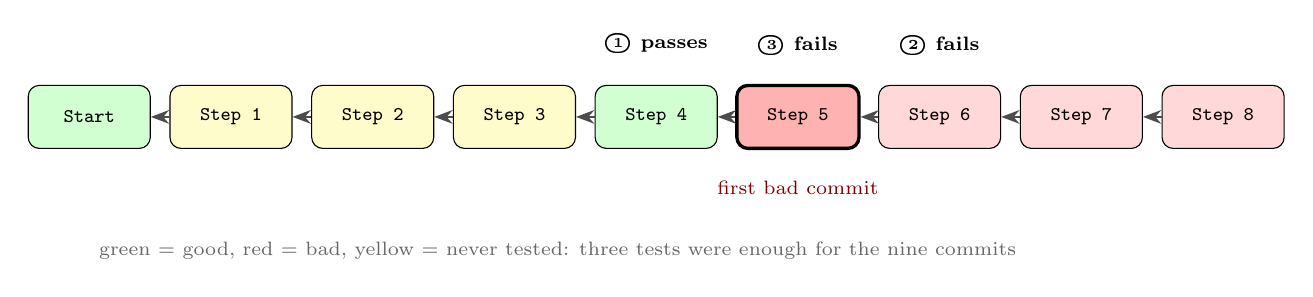
\begin{tikzpicture}
  \node[goodc] (s0) at (0,0) {Start}; \node[unkc] (s1) at (1.8,0) {Step 1}; \node[unkc] (s2) at (3.6,0) {Step 2}; \node[unkc] (s3) at (5.4,0) {Step 3};
  \node[goodc] (s4) at (7.2,0) {Step 4}; \node[badc,fill=red!30,very thick] (s5) at (9.0,0) {Step 5}; \node[badc] (s6) at (10.8,0) {Step 6}; \node[badc] (s7) at (12.6,0) {Step 7}; \node[badc] (s8) at (14.4,0) {Step 8};
  \foreach \a/\b in {s1/s0,s2/s1,s3/s2,s4/s3,s5/s4,s6/s5,s7/s6,s8/s7} { \draw[link] (\a)--(\b); }
  \node[font=\scriptsize\bfseries] at (7.2,0.9) {\textcircled{\tiny 1} passes};
  \node[font=\scriptsize\bfseries] at (10.8,0.9) {\textcircled{\tiny 2} fails};
  \node[font=\scriptsize\bfseries] at (9.0,0.9) {\textcircled{\tiny 3} fails};
  \node[font=\scriptsize,text=red!50!black] at (9.0,-0.9) {first bad commit};
  \node[font=\scriptsize,text=black!60,align=left,anchor=west] at (0,-1.7) {green = good, red = bad, yellow = never tested: three tests were enough for the nine commits};
\end{tikzpicture}
\caption{The search of the demo: test \textcircled{\tiny 1} \code{Step 4} (good), \textcircled{\tiny 2} \code{Step 6} (bad), \textcircled{\tiny 3} \code{Step 5} (bad). Since \code{Step 4} is good and \code{Step 5} is bad, \code{Step 5} is the culprit.}
\label{fig:bisect}
\end{figure}

\begin{pitfall}
Always finish with \code{git bisect reset}; until then you are on a temporary, detached state (Lecture 4). Bisect needs a \emph{reliable} test (the same result every time), and a commit that cannot be tested at all can be skipped with \code{git bisect skip}.
\end{pitfall}

\section{Under the hood: what is inside \texttt{.git}?}

You have used Git for ten lectures; now look inside. The hidden folder from Lecture 1 is a small database plus a few pointer files:

\begin{lstlisting}
$ ls .git
COMMIT_EDITMSG  HEAD  ORIG_HEAD  config  description  hooks  index
info  logs  objects  refs
$ cat .git/HEAD
ref: refs/heads/main
$ cat .git/refs/heads/main
6529ff1c759ea9c51798a7e5852fd5f21964cb57
\end{lstlisting}

\begin{itemize}
  \item \code{HEAD} is a one-line file: ``I am on branch \code{main}'' (Lecture 4's picture, literally).
  \item A \textbf{branch} is a file containing a commit ID: 40 characters, nothing else. That is why creating a branch costs nothing. (After a clone or a \code{git gc} you may also see a file \code{packed-refs}: Git's tidy summary of many such files, in which case the branch's file can be missing.)
  \item \code{index} is the staging area. \code{logs} is the reflog. \code{config} holds the local settings of Lecture 1. \code{hooks} can hold scripts that Git runs at certain moments.
  \item \code{objects} is the database of everything you ever committed.
\end{itemize}

\subsection{Four kinds of objects}

Everything in \code{objects} is one of four kinds, each stored under the \textbf{hash} of its contents:

\begin{center}
\small
\begin{tabular}{@{}l >{\raggedright\arraybackslash}p{10.8cm}@{}}
\toprule
Object & What it holds \\
\midrule
\textbf{blob} & the contents of one file (no name, no folder) \\
\textbf{tree} & a folder: a list of names, each pointing to a blob (file) or another tree (subfolder) \\
\textbf{commit} & a pointer to one tree (the snapshot), the parent commit(s), author, date, message \\
\textbf{tag} & an annotated tag (Lecture 9): a name, a message, and a pointer to a commit \\
\bottomrule
\end{tabular}
\end{center}

You can look at them with \code{git cat-file}:

\begin{lstlisting}
$ git cat-file -t HEAD
commit
$ git cat-file -p HEAD
tree aeba1480b8783d748b9cd09f5ad0cbc64f127587
parent 9d18d71a8420fffe8667946d288bfd39d1ef5fd7
author Practice User <practice@example.com> 1738659600 +0000
committer Practice User <practice@example.com> 1738659600 +0000

Add waffle recipe
$ git cat-file -p HEAD^{tree}
100644 blob ae5e354863163528256fab6c692aaada622e83bd	README.md
100644 blob 010497540ae142ff657f07122465b4fc646c4bb1	recipes.txt
$ git cat-file -p HEAD:recipes.txt
Pancakes: flour, milk, eggs
Crepes: flour, milk, eggs, butter
Waffles: flour, milk, eggs, sugar
\end{lstlisting}

A commit is thus tiny: a tree ID, a parent ID, who and when. The ``snapshot'' of Lecture 2 is the tree it points to.

\begin{figure}[H]
\centering
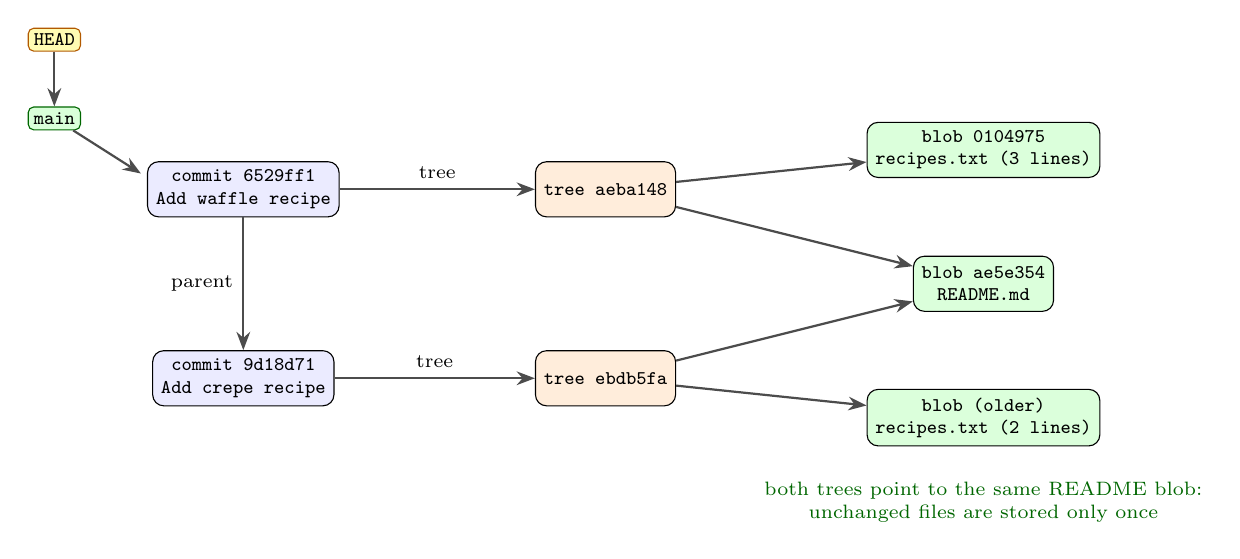
\begin{tikzpicture}
  \node[obj,fill=blue!8] (c2) at (0,0) {commit 6529ff1\\\scriptsize Add waffle recipe};
  \node[obj,fill=blue!8] (c1) at (0,-2.4) {commit 9d18d71\\\scriptsize Add crepe recipe};
  \node[obj,fill=orange!14] (t2) at (4.6,0) {tree aeba148};
  \node[obj,fill=orange!14] (t1) at (4.6,-2.4) {tree ebdb5fa};
  \node[obj,fill=green!14] (b0) at (9.4,-1.2) {blob ae5e354\\\scriptsize README.md};
  \node[obj,fill=green!14] (b2) at (9.4,0.5) {blob 0104975\\\scriptsize recipes.txt (3 lines)};
  \node[obj,fill=green!14] (b1) at (9.4,-2.9) {blob (older)\\\scriptsize recipes.txt (2 lines)};
  \draw[link] (c2)--node[above,font=\scriptsize,text=black]{tree}(t2); \draw[link] (c1)--node[above,font=\scriptsize,text=black]{tree}(t1);
  \draw[link] (c2)--node[left,font=\scriptsize,text=black]{parent}(c1);
  \node[branchtag] (mn) at (-2.4,0.9) {main}; \node[headtag] (hd) at (-2.4,1.9) {HEAD};
  \draw[link] (mn)--(-1.3,0.2); \draw[link] (hd)--(mn);
  \draw[link] (t2)--(b2); \draw[link] (t2)--(b0); \draw[link] (t1)--(b0); \draw[link] (t1)--(b1);
  \node[font=\scriptsize,text=green!40!black,anchor=north,align=center] at (9.4,-3.6) {both trees point to the same README blob:\\unchanged files are stored only once};
\end{tikzpicture}
\caption{Two commits as stored objects. The README did not change, so both trees point to the very same blob.}
\label{fig:objects}
\end{figure}

\subsection{Why IDs behave the way they do}

The ID of an object is a \textbf{hash} (SHA-1, 40 hexadecimal characters) of its content. Same content, same ID, anywhere in the world:

\begin{lstlisting}
$ echo "hello" | git hash-object --stdin
ce013625030ba8dba906f756967f9e9ca394464a
\end{lstlisting}

This one idea explains much of what you learned:
\begin{itemize}
  \item \emph{Unchanged files are stored once} (Figure~\ref{fig:objects}): same content, same blob.
  \item \emph{Rebase makes ``copies'' with new IDs} (Lecture 8): a commit contains its parent's ID, so a different parent means different content, hence a different hash.
  \item \emph{History cannot be changed silently}: altering an old commit changes its ID and every ID after it.
  \item \emph{Branches are cheap}: just a file with an ID in it.
\end{itemize}

Objects that nothing points to (the ``lost'' commits of the reflog section) are \emph{unreachable}; \code{git gc} removes them after their reflog entries have expired. (Git also packs many loose objects into compact \emph{pack files}; newer Git can even use SHA-256 instead of SHA-1: the ideas stay the same, only the IDs differ. You rarely need to think about either.)

\section{Which command for which situation?}

\begin{center}
\small
\begin{tabular}{@{}>{\raggedright\arraybackslash}p{6.4cm} >{\raggedright\arraybackslash}p{6.3cm}@{}}
\toprule
I want to\ldots & Use (lecture) \\
\midrule
see where I am and what changed & \code{git status}, \code{git diff}, \code{git log --oneline --graph} (2, 3, 4) \\
undo an unstaged or staged change & \code{git restore file}, \code{git restore --staged file} (3) \\
fix my last commit (unshared) & \code{git commit --amend} (3) \\
undo a shared commit safely & \code{git revert} (3) \\
work on an idea separately & \code{git switch -c name} (4) \\
combine branches & \code{git merge}; fix conflicts, \code{git add}, commit (5) \\
share, download & \code{push}, \code{fetch}, \code{pull}, \code{clone} (6) \\
propose a change & branch, push, pull request (7) \\
tidy my unshared commits & \code{git rebase -i}, \code{reset --soft} (8, 10) \\
copy one commit & \code{git cherry-pick} (8) \\
find a lost commit & \code{git reflog}, then \code{git branch rescue <id>} (10) \\
park unfinished work & \code{git stash push -m} / \code{pop} / \code{apply} (10) \\
undo a fresh merge, rebase or reset & \code{git reset --hard ORIG\_HEAD} (10) \\
look at an old commit & \code{git switch --detach <id>} (4) \\
find the commit that broke it & \code{git bisect run} (10) \\
name a version & \code{git tag -a}, release (9) \\
\bottomrule
\end{tabular}
\end{center}

\section{Where to go from here}

You can now do everything a working developer does with Git every day. To keep growing:

\begin{itemize}
  \item \textbf{Practise on real projects.} Use Git for your own notes, papers or code from today on. Commit small, read \code{git status} before and after every command, make a branch for every idea.
  \item \textbf{Contribute.} Look for the label \emph{good first issue}; \code{firstcontributions/first-contributions} on GitHub is a safe first pull request.
  \item \textbf{Read.} \emph{Pro Git} (free at \url{https://git-scm.com/book}) goes deeper on every topic; \code{git help <command>} is always at hand.
  \item \textbf{Play.} \url{https://learngitbranching.js.org} shows branches and rebases as animated pictures. \url{https://ohshitgit.com} lists rescue recipes for common mistakes. \url{https://skills.github.com} offers short interactive GitHub courses.
  \item \textbf{Discover more tools:} \code{git blame} (who wrote this line?), \code{git log -S"text"} (when did this text appear?), aliases, hooks, submodules, Git LFS, signed commits.
\end{itemize}

\begin{keyidea}
Four habits cover most of Git: \textbf{commit small and often; read \code{git status}; branch for every idea; never rewrite what others have}. If you break the last one by accident, \code{git reflog} is your friend.
\end{keyidea}

\Needspace{12\baselineskip}
\section{Homework 10}

\begin{homework}{10: Rescue, squash, bisect, shelve}
The setup script builds \code{practice/hw10}: a repository where two commits were lost by a hard reset, a branch of messy commits, an urgent bug, and a chain of commits with a hidden bug. From the course folder:
\begin{lstlisting}
$ bash codeHints/L10/setup_hw10.sh
$ cd practice/hw10
\end{lstlisting}
Do the tasks in order. To start over: \code{setup\_hw10.sh --reset} from the course folder. Set your identity (\code{git config user.name} and \code{user.email}) if it is not set globally.

\begin{description}[leftmargin=1.2em,style=nextline]
\item[10.1 Rescue] On \code{main}, two commits including one called \code{Important work} were lost by a hard reset. Find it with \code{git reflog} (the reflog is long: press \code{q} to leave the pager, or filter it with \code{git reflog | grep Important}) and create a branch \code{rescued} that points at the commit named exactly \code{Important work} (\code{Start important work} is a different, older commit). Do \emph{not} move \code{main}.
\item[10.2 Squash] The branch \code{messy} has three commits (\code{wip}, \code{wip 2}, \code{more wip}) on top of \code{main}. Using \code{git reset --soft}, turn them into \emph{one} commit called \code{Add feature} with exactly the same files.
\item[10.3 Bisect] The branch \code{history} is a chain of 12 commits; a bug appeared at some step. Its first commit (\code{git rev-list --max-parents=0 history}) is good, its newest is bad, and \code{test.sh} in the repository tells good from bad. Use \code{git bisect run bash test.sh} to find the first bad commit, finish with \code{git bisect reset}, and write \code{bad-commit=<first 7 characters of its ID>} in \code{practice/hw10\_answers.txt} (next to \code{hw10}; use \code{printf} or \code{echo}).
\Needspace{7\baselineskip}
\item[10.4 Stash] Switch to \code{main}. Append the line \code{work in progress} to \code{notes.txt} and \emph{do not commit}. Now an urgent bug arrives: the branch \code{urgent} has the typo \code{teh} in \code{app.txt}. Shelve your change with \code{git stash}, switch to \code{urgent}, fix the typo, commit it as \code{Fix urgent bug}, switch back to \code{main}, and \code{git stash pop}. At the end \code{git status --short} must show only \code{\ M notes.txt} (a space, then \code{M}) and the stash must be empty.
\item[10.5 Look inside] Add three more lines to the answers file: \code{tree=<first 7 characters of the ID of main's tree>} (use \code{git cat-file -p main}), \code{hello=<first 7 characters of the hash of the text hello>} (use \code{printf 'hello\textbackslash n' | git hash-object --stdin}; run this in Git Bash, other shells may add different line endings), and \code{ref-file=<first 7 characters stored in .git/refs/heads/main>} (use \code{cat}; if the file does not exist, Git has packed it, so use \code{git rev-parse main} instead).
\end{description}

\textbf{Check yourself:} from the course folder run \code{bash codeHints/L10/check\_hw10.sh}. All \code{PASS}, then compare with the solutions at the end of this lecture (or in \code{solutions/L10/}).
\end{homework}

\section{Summary and farewell}

\begin{itemize}
  \item Committed work is almost never lost: \code{git reflog} lists where \code{HEAD} has been; \code{git branch rescue <id>} saves a lost commit. \code{ORIG\_HEAD} undoes a fresh merge, rebase or reset.
  \item \code{reset --soft/--mixed/--hard} move the branch and keep, unstage, or discard your changes. \code{--hard} destroys uncommitted work; never reset shared history.
  \item \code{git stash} shelves uncommitted work; \code{git bisect run} finds the commit that broke something by binary search.
  \item Inside \code{.git}: branches are files holding IDs, commits point to trees, trees to blobs, and every ID is a hash of content.
\end{itemize}

\textbf{You have finished the course.} In Lecture 0 we started with a folder full of \code{report\_v2\_final\_}\allowbreak\code{REALLY\_final.docx} files and asked for a time machine and a collaboration tool. You now have both: from \code{git init} to rebase, pull requests and recovery. Keep the four habits, keep practising, and enjoy using Git. (\emph{Pro Git}, Chapters 7.3 and 10.)

\solutionspage

\section*{Solutions to Homework 10}

\begin{lstlisting}
$ bash codeHints/L10/setup_hw10.sh
$ cd practice/hw10
$ git reflog | grep "Important work"            # 10.1
0b30b44 HEAD@{18}: commit: Important work
$ git branch rescued 0b30b44                      # use the ID you see
$ git switch messy                                # 10.2
$ git reset --soft main
$ git commit -m "Add feature"
$ git switch history                              # 10.3
$ git bisect start
$ git bisect bad
$ git bisect good $(git rev-list --max-parents=0 history)
$ git bisect run bash test.sh
... is the first bad commit
$ git bisect reset
$ git switch main                                 # 10.4
$ echo "work in progress" >> notes.txt
$ git stash
$ git switch urgent
$ sed -i.bak 's/teh/the/' app.txt && rm app.txt.bak     # or edit by hand
$ git commit -am "Fix urgent bug"
$ git switch main
$ git stash pop
$ git status --short
 M notes.txt
\end{lstlisting}

For 10.5 (the three IDs are examples, yours differ except the hash of \code{hello}):

\begin{lstlisting}
$ git cat-file -p main | head -1
tree 8cfff4b...
$ echo hello | git hash-object --stdin
ce013625030ba8dba906f756967f9e9ca394464a
$ cat .git/refs/heads/main
1689350...
$ printf 'bad-commit=e238140\ntree=8cfff4b\nhello=ce01362\nref-file=1689350\n' > ../hw10_answers.txt
\end{lstlisting}

\textbf{10.1.} The reset moved \code{main} back, but the reflog remembers every position of \code{HEAD}. Your reflog is long because it also contains the history of the setup; \code{grep} finds the line. \code{git branch rescued <id>} only adds a label, so \code{main} stays where it was. (If you used \code{git reset --hard <id>} on \code{main}, the rescue works but \code{main} moved, and the checker complains.)

\textbf{10.2.} \code{git reset --soft main} moves \code{messy} back to \code{main}'s commit but keeps all the changes \emph{staged}, so a single \code{git commit} makes one commit with exactly the same files as the three wip commits (the checker compares the file contents).

\textbf{10.3.} \code{bisect run} tests about $\log_2 12 \approx 4$ commits. The first bad commit is \code{Step 7}. Do not forget \code{git bisect reset}: otherwise the repository stays in bisect mode and the checker reports it.

\textbf{10.4.} A stash lets you switch branches with a clean working directory. After the pop, your uncommitted line is back in \code{notes.txt}, and the commit \code{Fix urgent bug} lives on \code{urgent}, not on \code{main}. If \code{git stash pop} reports a conflict, you changed the same lines on both sides; resolve it as in Lecture 5.

\textbf{10.5.} \code{git cat-file -p main} prints a commit: its first line gives the ID of its tree. The hash of \code{hello} is the same on every computer (\code{ce01362\dots}). The file \code{.git/refs/heads/main} holds the full ID of \code{main}'s commit, so its first 7 characters equal \code{git rev-parse --short=7 main}. (If the file does not exist, Git has packed the reference into \code{.git/packed-refs}; use \code{git rev-parse main} instead.)

\Needspace{8\baselineskip}
\textbf{Common mistakes.}
\begin{itemize}
  \item Moving \code{main} to the lost commit in 10.1 instead of creating a branch.
  \item Forgetting \code{git bisect reset}; or running bisect while having uncommitted changes (stash or commit first).
  \item Committing the \code{work in progress} line instead of stashing it in 10.4: then \code{main} has a new commit and the check ``only \code{ M notes.txt}'' fails.
  \item Writing the \emph{whole} 40-character ID is fine, but the checker also needs at least 7 characters.
\end{itemize}


\end{document}
